\documentclass{article}
\usepackage{graphicx} % Required for inserting images
\usepackage{etoolbox}
\usepackage[letterpaper, margin=1in]{geometry}
\usepackage{fancyhdr}
\usepackage{longtable}
\usepackage{array}


\author{Antoine Legrain}

% nom et matricule sont redéfinis dans le fichier data.tex généré par le programme
\newcommand{\nom}{}
\newcommand{\widthratio}{.5}

\begin{document}

% Set the page style to "fancy"...
\pagestyle{fancy}
\fancyhead{} % clear all header fields
\renewcommand{\nom}{George}
\renewcommand{\widthratio}{0.50}

\fancyhead[L]{\nom}

\begin{longtable}{m{.15\textwidth}|m{.05\textwidth}|c}
    Questions & Notes & Boîte à moustache \\ \hline \hline
    1 & 5 & 2.5 & 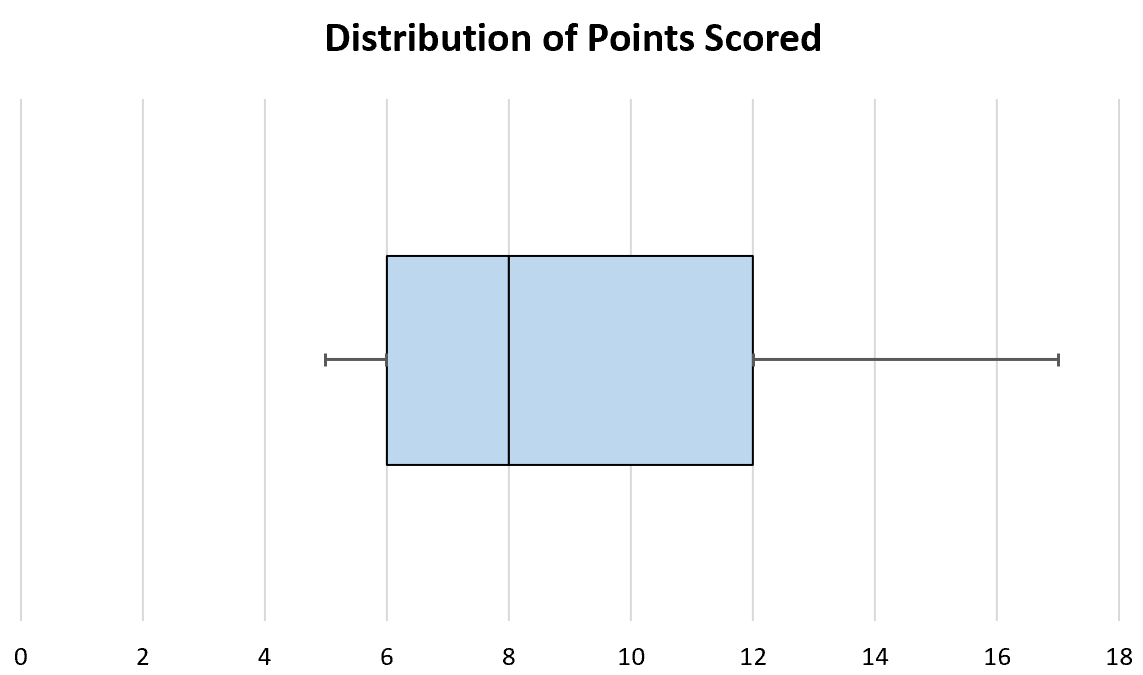
\includegraphics[width=\widthratio \textwidth]{boxplot.png} \\ \hline
Total (/ 10) & 5 & 2.5 & 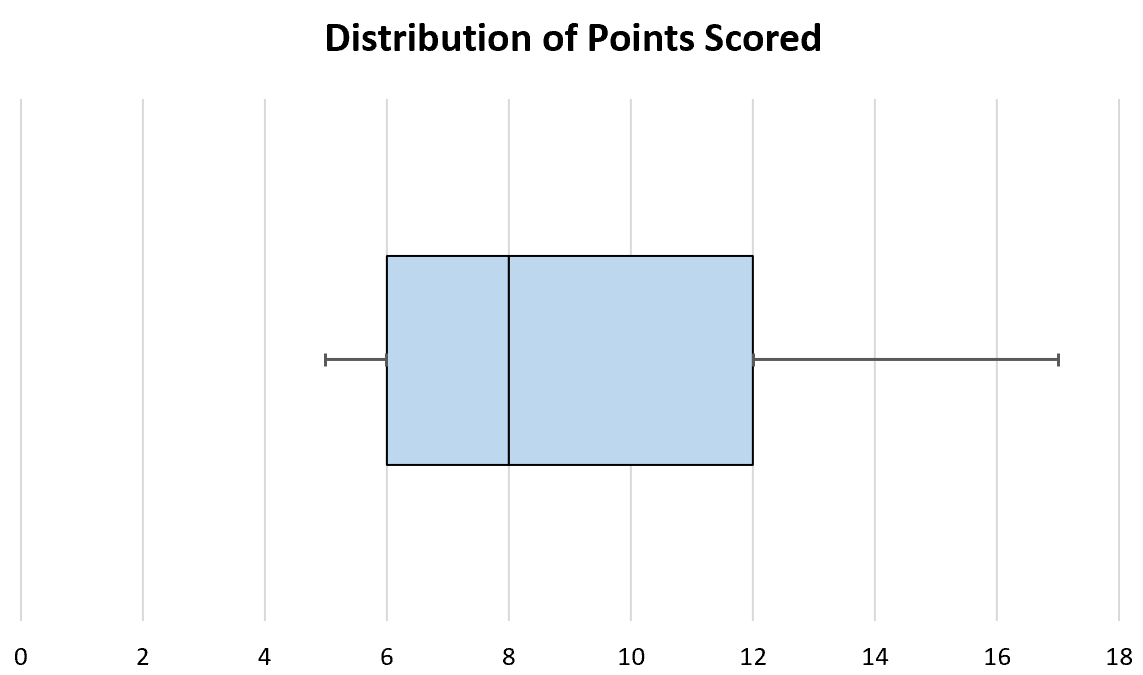
\includegraphics[width=\widthratio \textwidth]{boxplot.png}

\end{longtable}

\end{document}
